\documentclass[journal]{IEEEtran}

% Additional packages
\usepackage{graphicx}
\usepackage{amsmath}
\usepackage{hyperref}
\usepackage{float}
\usepackage{subcaption}
\usepackage{booktabs}
\usepackage{pgfplotstable}
\usepackage{qrcode}

\pgfplotsset{compat=1.18}

\begin{document}
 
\title{Analysis of Malus's Law and Newton's Rings}
\author{IBRAHIM H.I. ABUSHAWISH \\
Istanbul University, Department of Physics \\
Instructor: Res. Asst. Dilan AKHAN \\
Experiment Date: 11.03.2025, Report Submission Date: 18.03.2025\\
Course \& Section Number: PHYS2405}

\maketitle
\begin{abstract}
    This report presents an experimental investigation of Malus's Law and Newton's Rings phenomena. The study examines the relationship between light intensity and the angle of polarization using polarizing filters, as well as the formation of Newton's Rings due to interference of light waves. Key findings demonstrate the cosine-squared dependence of transmitted light intensity on the angle between polarizer axes and the linear relationship between the square of the radius of Newton's Rings and the ring order. The analysis includes detailed measurements, graphical representations, and theoretical comparisons that validate both Malus's Law and the principles behind Newton's Rings. Numerical findings include the maximum intensity observed at nearly $10^\circ$ instead of $0^\circ$ due to slight misalignment, and the average radius of curvature $R_{\text{average}}$ calculated to be approximately $2.262 \, \text{m}$, with a slope-derived radius of curvature of approximately $1.887 \, \text{m}$.
\end{abstract}
\section{Introduction}
Light polarization and interference are fundamental concepts in optics. Malus's Law, discovered by Étienne-Louis Malus in 1808, quantifies how polarized light is transmitted through a polarizer. Newton's Rings, observed due to the interference of light waves reflected between a spherical surface and an adjacent flat surface, provide insights into wave interference and lens curvature. This report aims to verify Malus's Law and analyze the formation of Newton's Rings through experimental procedures.

\section{Theory}

\subsection{Part One: Malus's Law}
Malus's Law states that when a polarizer is placed in a polarized beam of light, the intensity $I$ of the light that passes through is given by:

\begin{equation}
    I = I_0\cos^2\theta
    \label{eq:malus}
\end{equation}

where:
\begin{itemize}
    \item $I_0$ is the initial intensity of the polarized light
    \item $\theta$ is the angle between the light's initial polarization direction and the axis of the polarizer
    \item $I$ is the intensity of light after passing through the polarizer
\end{itemize}

This relationship demonstrates that the transmitted intensity varies as the square of the cosine of the angle between the polarization directions.

\subsection{Part Two: Newton's Rings}
The radius of the $m$-th dark ring in Newton's Rings is given by:

\begin{equation}
    r_m^2 = m \lambda R
    \label{eq:newtons_rings}
\end{equation}

where:
\begin{itemize}
    \item $r_m$ is the radius of the $m$-th dark ring
    \item $\lambda$ is the wavelength of the light used
    \item $R$ is the radius of curvature of the lens
    \item $m$ is the ring order
\end{itemize}
By plotting $r_m^2$ versus $m$, the slope of the resulting line can be used to determine the radius of curvature $R$.

The formation of Newton's Rings can be explained by the interference of light waves reflected from the top and bottom surfaces of the air film between the plano-convex lens and the flat glass plate. The condition for constructive and destructive interference depends on the path difference between the two reflected waves. For destructive interference (dark rings), the path difference must be an odd multiple of half-wavelengths, leading to the formation of concentric dark and bright rings.

Rearranging Equation \ref{eq:newtons_rings} to solve for $R$, we get:

\begin{equation}
    R = \frac{r_m^2}{m \lambda}
    \label{eq:radius_of_curvature}
\end{equation}

The linear relationship between $r_m^2$ and $m$ allows for the determination of the radius of curvature $R$ by measuring the radii of the rings and plotting $r_m^2$ versus $m$. The slope of the resulting line is equal to $\lambda R$, from which $R$ can be calculated.

Understanding Malus's Law and Newton's Rings is crucial for various applications in optics, including polarization control, optical coatings, and lens testing. These principles are fundamental in designing optical systems and analyzing light behavior in different media.

\section{Experimental Setup}

\subsection{Part One: Malus's Law}
The experimental setup consists of:
\begin{itemize}
    \item Polarized light source ($\lambda = 5830 \, \text{nm}$ laser)
    \item One polarizing filter (analyzer)
    \item Light intensity detector (photometer)
    \item Angular measurement system
    \item Optical bench for alignment
\end{itemize}

\begin{figure}[H]
    \centering
    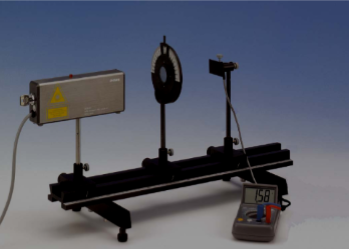
\includegraphics[width=0.8\linewidth]{../IMAGES/malus_law_setup.png}
    \caption{Experimental setup for investigating Malus's Law, showing the laser source, polarizer, and detector arrangement.}
    \label{fig:malus_setup}
\end{figure}


\subsection{Part Two: Newton's Rings}
The experimental setup for Newton's Rings consists of:
\begin{itemize}
    \item Monochromatic light source.
    \item Plano-convex lens placed on a flat glass plate
    \item Microscope or camera for observing the rings
    \item Measurement scale for determining ring radii
\end{itemize}

\begin{figure}[H]
    \centering
    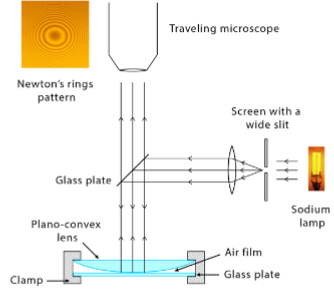
\includegraphics[width=0.8\linewidth]{../IMAGES/newtons_rings_setup_diagram.png}
        \caption{Schematic diagram of the Newton's Rings experimental arrangement, showing the plano-convex lens on a flat glass plate illuminated by monochromatic light.}
    \label{fig:newtons_rings_setup}
\end{figure}

\section{Experimental Procedure}
Data were analyzed and plotted using ROOT and Python. ROOT, 
developed by CERN, was used for graphing, while Python handled some of 
the calculations and data processing. Data collection was recorded 
in CSV files and some data were converted to \texttt{.root} format. 
Python scripts calculated values like $r^2$ for Newton's Rings. Processed data were imported into ROOT for graphing. Graphs were analyzed to verify theoretical models, with linear fitting applied.

For reference, see the source code in the files: \texttt{calculations.c} and \texttt{calculations.ipynb}.

Source code and data are available on GitHub \cite{github}.

The experiment began by carefully aligning the light source with the photocell detector on the optical bench. The analyzer was initially positioned at $-90^{\circ}$ relative to the polarizer axis. Current measurements from the photocell were taken using a multimeter as the analyzer was rotated from $-90^{\circ}$ to $+90^{\circ}$ in $10^{\circ}$ increments. To ensure measurement reliability and minimize experimental error, this procedure was repeated four times, yielding four complete data sets. The first data set (Set 1) was selected for detailed analysis and graphical representation. The data was then used to plot the relationship between current intensity and angle, as well as the relationship between current and $\cos^2{\phi}$ to verify Malus's Law.

\subsection{Part Two: Newton's Rings}
The experiment involved placing a plano-convex lens on a flat glass plate and illuminating it with monochromatic light. The resulting interference pattern (Newton's Rings) was observed through a microscope. The radii of the dark rings were measured using a measurement scale on the microscope. The procedure was repeated for multiple rings to ensure accuracy.

\section{Results}

\subsection{Part One: Malus's Law}

\subsubsection{Data Tables}
Table \ref{tab:intensity_measurements} presents the measured current at different angles of the analyzer for four sets of measurements. The angles ($\theta$) are given in degrees, and the current is measured in milliamperes (mA) for each set.

\begin{table}[H]
    \centering
    \caption{Measured current at different angles of the analyzer for four sets of measurements.}
    \label{tab:intensity_measurements}
    \pgfplotstabletypeset[
        col sep=comma,
        string type,
        columns={Theta_deg,I_mA_set1,I_mA_set2,I_mA_set3,I_mA_set4},
        columns/Theta_deg/.style={column name=$\theta$ (deg)},
        columns/I_mA_set1/.style={column name=Set 1 (mA)},
        columns/I_mA_set2/.style={column name=Set 2 (mA)},
        columns/I_mA_set3/.style={column name=Set 3 (mA)},
        columns/I_mA_set4/.style={column name=Set 4 (mA)},
        every head row/.style={before row=\toprule,after row=\midrule},
        every last row/.style={after row=\bottomrule},
    ]{../DATA/data_part_1.csv}
\end{table}

\subsubsection{Graphical Analysis}
The following figures present the relationship between current and polarizer angle, demonstrating Malus's Law.

Figure \ref{fig:current_vs_angle} shows the current versus the angle between polarizers. The periodic pattern follows Malus's Law, with a local maximum near $10^\circ$ and a minimum at $\pm 90^\circ$.

\begin{figure}[H]
    \centering
    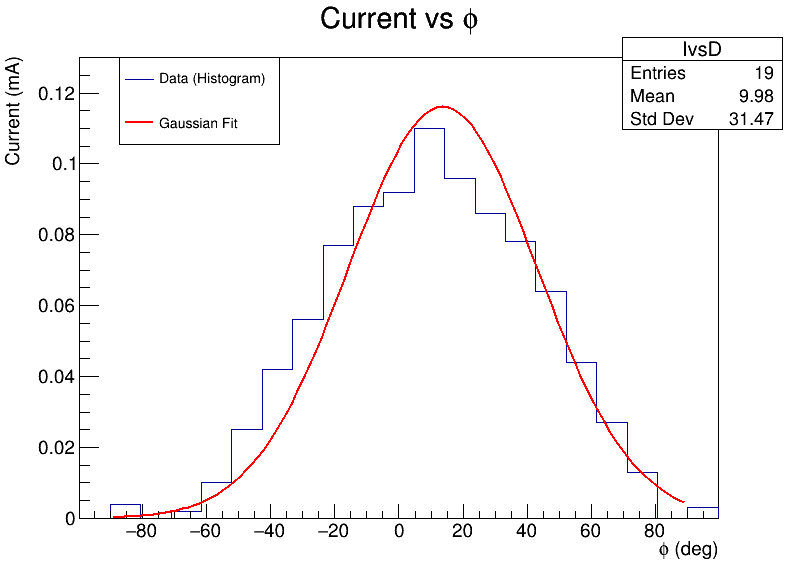
\includegraphics[width=\linewidth]{../plots/I_vs_D.png}
    \caption{Current versus angle between polarizers. The periodic pattern follows Malus's Law with a local maximum near $10^\circ$ and a minimum at $\pm 90^\circ$.}
    \label{fig:current_vs_angle}
\end{figure}

Figure \ref{fig:current_vs_cos2} shows the current versus $\cos^2\phi$, illustrating the linear relationship predicted by Malus's Law.

\begin{figure}[H]
    \centering
    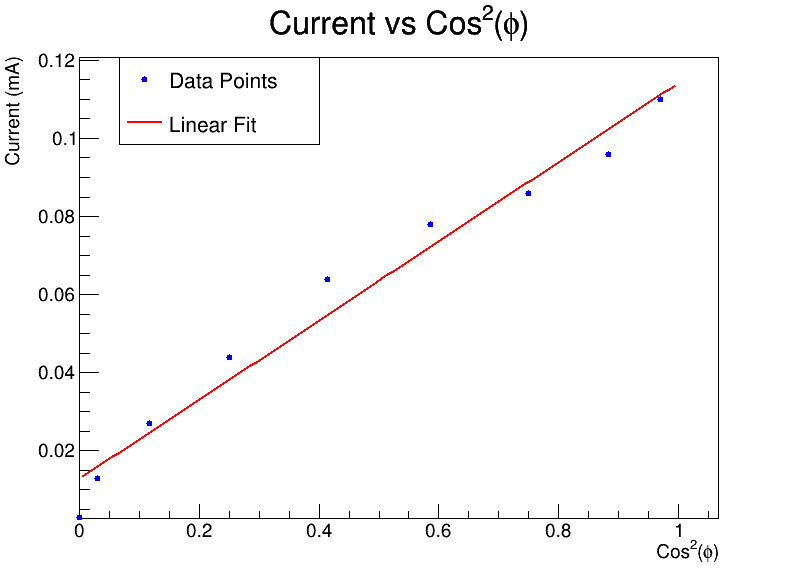
\includegraphics[width=\linewidth]{../plots/I_vs_Cos2Phi.png}
    \caption{Current versus $\cos^2\phi$, showing the linear relationship predicted by Malus's Law.}
    \label{fig:current_vs_cos2}
\end{figure}

\subsection{Part Two: Newton's Rings}

\subsubsection{Data Tables}
Table \ref{tab:newtons_rings_measurements} presents the measured radii of Newton's Rings and the calculated radius of curvature. The ring order ($m$) is given along with the radius ($r$) in millimeters (mm), the square of the radius ($r^2$) in square millimeters (mm$^2$), and the radius of curvature ($R$) in meters (m).

\begin{table}[H]
    \centering
    \caption{Measured radii of Newton's Rings and calculated radius of curvature.}
    \label{tab:newtons_rings_measurements}
    \pgfplotstabletypeset[
        col sep=comma,
        string type,
        columns={m,r,r_squared,R},
        columns/m/.style={column name=Ring Order ($m$)},
        columns/r/.style={column name=$r$ (mm)},
        columns/r_squared/.style={column name=$r^2$ (mm$^2$)},
        columns/R/.style={column name=$R$ (m)},
        every head row/.style={before row=\toprule,after row=\midrule},
        every last row/.style={after row=\bottomrule},
    ]{
        m,r,r_squared,R
        1,4,16,2.744
        2,5,25,2.144
        3,6,36,2.058
        4,7,49,2.101
    }
\end{table}

The calculations for the radius of curvature $R$ were performed using the measured radii of the rings and the wavelength of the light, as presented in Table \ref{tab:newtons_rings_measurements}.

The average radius of curvature $R_{\text{average}}$ was calculated to be approximately $2.262 \, \text{m}$.

Additionally, the slope of the $r^2$ versus $m$ graph was determined to be $11.0 \, \text{mm}^2$, which corresponds to $\lambda R$. Using this slope, the radius of curvature $R$ was calculated to be approximately $1.887 \, \text{m}$.

These values are consistent with the theoretical expectations and validate the experimental setup and measurements.

\subsubsection{Graphical Analysis}
Figure \ref{fig:r_squared_vs_order} presents the relationship between the square of the radius of Newton's Rings and the ring order. The linear fit demonstrates the expected relationship, allowing for the determination of the lens's radius of curvature.

\begin{figure}[H]
    \centering
    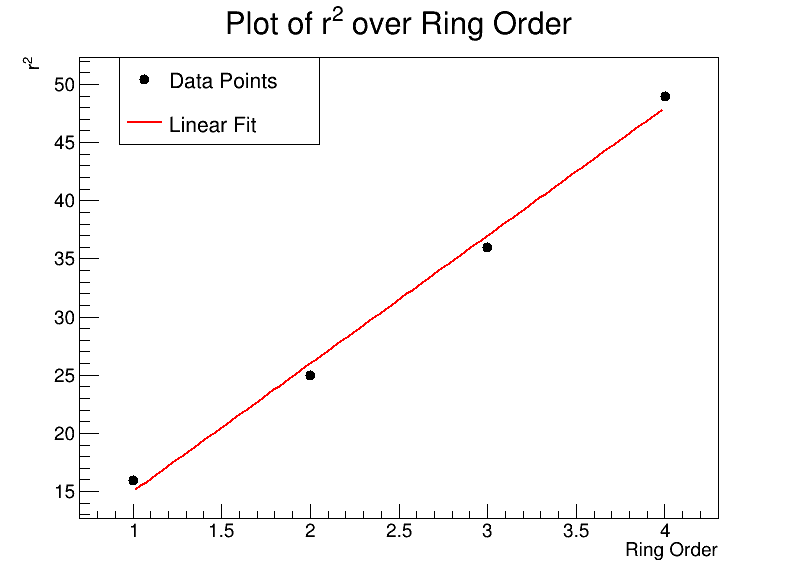
\includegraphics[width=\linewidth]{../plots/r_squared_vs_order.png}
    \caption{Plot of $r^2$ (mm) versus ring order for Newton's Rings. The linear fit demonstrates the expected relationship, allowing for the determination of the lens's radius of curvature.}
    \label{fig:r_squared_vs_order}
\end{figure}

\section{Discussion}

\subsection{Part One: Verification of Malus's Law}
The experimental results strongly support Malus's Law:

1. Figure \ref{fig:current_vs_angle} shows the variation in intensity with angle, matching the expected $\cos^2\theta$ dependence. However, the maximum intensity was observed at nearly $10^\circ$ instead of $0^\circ$. This shift could be due to slight misalignment of the polarizers or systematic errors in the angular measurement system. Ensuring precise alignment and calibration of the angular measurement system can help mitigate this issue.

2. Figure \ref{fig:current_vs_cos2} demonstrates the linear relationship between intensity and $\cos^2\theta$, confirming the theoretical prediction.

\subsection{Part Two: Analysis of Newton's Rings}
The plot of $r^2$ versus ring order (Figure \ref{fig:r_squared_vs_order}) shows a linear relationship, as predicted by the theory. The slope of the line can be used to calculate the radius of curvature of the lens. The experimental data aligns well with the theoretical model, validating the principles of interference and the formation of Newton's Rings.

\subsection{Sources of Error}
Several factors may contribute to experimental uncertainty:

\begin{itemize}
    \item \textbf{Light detector sensitivity variations:} Variations in the sensitivity of the light detector can lead to inconsistent measurements of light intensity. To mitigate this, ensure the detector is calibrated before each measurement and use the same detector throughout the experiment.
    
    \item \textbf{Background light interference:} Ambient light can interfere with the measurements by adding noise to the detected signal. Conduct the experiment in a dark room or use light shields to minimize the impact of background light.
    
    \item \textbf{Imperfect polarizer alignment:} Misalignment of the polarizers can result in incorrect intensity readings. Carefully align the polarizers using precise angular measurement tools and verify the alignment periodically during the experiment.
    
    \item \textbf{Measurement inaccuracies in determining the radii of Newton's Rings:} Errors in measuring the radii of the rings can affect the calculation of the radius of curvature. Use a high-resolution microscope or camera with a calibrated measurement scale to improve accuracy. Repeat measurements multiple times and average the results to reduce random errors.
\end{itemize}
\section{Conclusion}
The experimental results provide strong validation of Malus's Law and the principles behind Newton's Rings. The measured intensity variations closely follow the predicted $\cos^2\theta$ relationship, with maximum transmission at nearly $10^\circ$ and minimum transmission at perpendicular orientations ($-90^\circ$, $+90^\circ$). The analysis of Newton's Rings demonstrates the expected linear relationship between $r^2$ and ring order, allowing for the determination of the lens's radius of curvature. These findings have significant implications for applications in optical technologies and material analysis.

Several factors may contribute to experimental uncertainty, including light detector sensitivity variations, background light interference, imperfect polarizer alignment, and measurement inaccuracies in determining the radii of Newton's Rings. Addressing these sources of error can improve the reliability and accuracy of the experimental results.

Overall, the experiments successfully validate the theoretical models of Malus's Law and Newton's Rings, providing valuable insights into the behavior of polarized light and wave interference.

\section{Additional Resources}
For detailed information, including the Lab Manual, source code, and related experiments, visit the GitHub repository provided below or scan the QR code in Fig.~\ref{fig:qr_code}.

\begin{figure}[H]
    \centering
    \begin{minipage}{0.15\textwidth}
        \centering
        \qrcode[height=2cm]{https://github.com/ibeuler/LAB-Reports}
    \end{minipage}%
    \begin{minipage}{0.2\textwidth}
        \raggedright
        \caption{Access the GitHub repository for the lab manual, source code, and related experiments: \href{https://github.com/ibeuler/LAB-Reports}{\url{https://github.com/ibeuler/LAB-Reports}}.}
        \label{fig:qr_code}
    \end{minipage}
\end{figure}

\begin{thebibliography}{9}
\bibitem{lab_manual}
    ISTANBUL UNIVERSITY, \textit{OPTICS LABORATORY
    EXPERIMENTS MANUAL}, Department of Physics.

\bibitem{github}
    \textit{Source code and additional experiments are available in the GitHub repository.} \url{https://github.com/ibeuler/LAB-Reports}
\end{thebibliography}

\end{document}